%!TEX root = ../thesis.tex

\chapter{Методи та підходи вирішення задач класифікації}
\label{chap:review}  %% відмічайте кожен розділ певною міткою -- на неї наприкінці необхідно посилатись

В даному розділі будуть основні теоретичні відомості про об'єкт дослідження та огляд суміжних робіт в даній сфері.

\section{Задача класифікації: визначення, види}

Класифікація — це процес віднесення об'єкту до певної категорії або класу на основі його характеристик, серед заздалегідь встановленого набору категорій. Класифікація може бути бінарною, багатокласовою, багатомітковою, ієрархічною та інші. Бінарна класифікація - це класифікація, коли кожному об'єкту обирається група з наперед визначеної множини груп в якій знаходиться рівно дві групи; багатокласова класифікація - це класифікація, коли кожному об'єкту обирається група з наперед визначеної множини груп в якій може знаходиться довільна кількість груп. В поточній роботі ми зосередимося на бінарній та багатокласовій класифікації.

Задача класифікації зустрічається в багатьох сферах, наприклад: медицина (діагностика раку на основі зображень МРТ), фінанси (класифікація позичальників як \glqq надійних\grqq\ чи \glqq ризикованих\grqq\ на основі їхньої кредитної історії), роздрібна торгівля (класифікація покупців за типами покупок для надання персоналізованих знижок), транспорт (розрізнення між легковими авто, вантажівками та мотоциклами на дорозі), освіта (ідентифікація студентів, яким потрібна додаткова допомога в певних предметах), безпека (класифікація електронних листів як \glqq безпечні,\grqq\ \glqq спам\grqq\ або \glqq фішинг\grqq), біотехнології (розпізнавання мутацій, що спричиняють хвороби). 

\section{Способи вирішення задачі класифікації}

Існує декілька способів для вирішення задачі класифікації: класичні статистичні методи (наприклад, логістична регресія~\cite{ct1}), алгоритми машинного навчання (наприклад, метод k-найближчих сусідів~\cite{ct4}), глибинне навчання (за допомогою нейронних мереж), а також задачу класифікації можна вирішувати за допомогою генетичних алгоритмів. Розглянемо більш детально, як працює глибинне навчання та генетичні алгоритми, розглядати детально, як працюють алгоритми класичного навчання ми не будемо, оскільки вони дуже різні, тому важко описати загальну концепцію, як вони працюють, оскільки в кожного алгоритму вона своя, але в наступному розділі я надам перелік основних алгоритмів та посилання на статті, де про них можна прочитати. 

Почнемо розгляд з глибинного навчання. В глибинному навчанні алгоритмами для вирішення задач є нейронні мережі. Нейромережі бувають дуже багатьох видів, але ми будемо їх розглядати на прикладі багатошарового перцептрону, оскільки саме його ми і використовуємо для експериментів. Багатошаровий перцептрон складається з шарів нейронів. Кожен нейрон в шарі, приймає якісь вхідні дані з попереднього шару, та обчислює вихідний сигнал, який передається наступному шару. Загалом те, що робить один нейрон можна описати наступною формулою:
\begin{equation}
\label{eq:neuron}
	a = f\left(\sum_{i=1}^n w_i x_i + b \right)
\end{equation}

де \(x_1, x_2, \ldots, x_n\) — вхідні сигнали до нейрону; \(w_1, w_2, \ldots, w_n\) — ваги, що призначені для кожного вхідного сигналу; \(b\) — зсув (англ. bias), що додається до суми зважених вхідних сигналів; \(f\) — активаційна функція, що може бути сигмоїдою, ReLU, тангенсом гіперболічним та іншими. В нейронній мережі може бути довільна кількість шарів та в кожному шарі може бути довільна кількість нейронів. Але усі вони працюють по вище наведеному принципу: на вхід кожному нейрону в кожному шарі приходить сигнал з попереднього шару і кожний нейрон генерує вихід, якщо це перший шар, то на вхід даються самі дані. Загалом схема нейронної мережі може виглядати наступним чином рисунок \ref{fig_nn_arch} в якому кожний круг це один нейрон, який розраховує функцію (\ref{eq:neuron}).

\begin{figure}[ht]
	\centering
	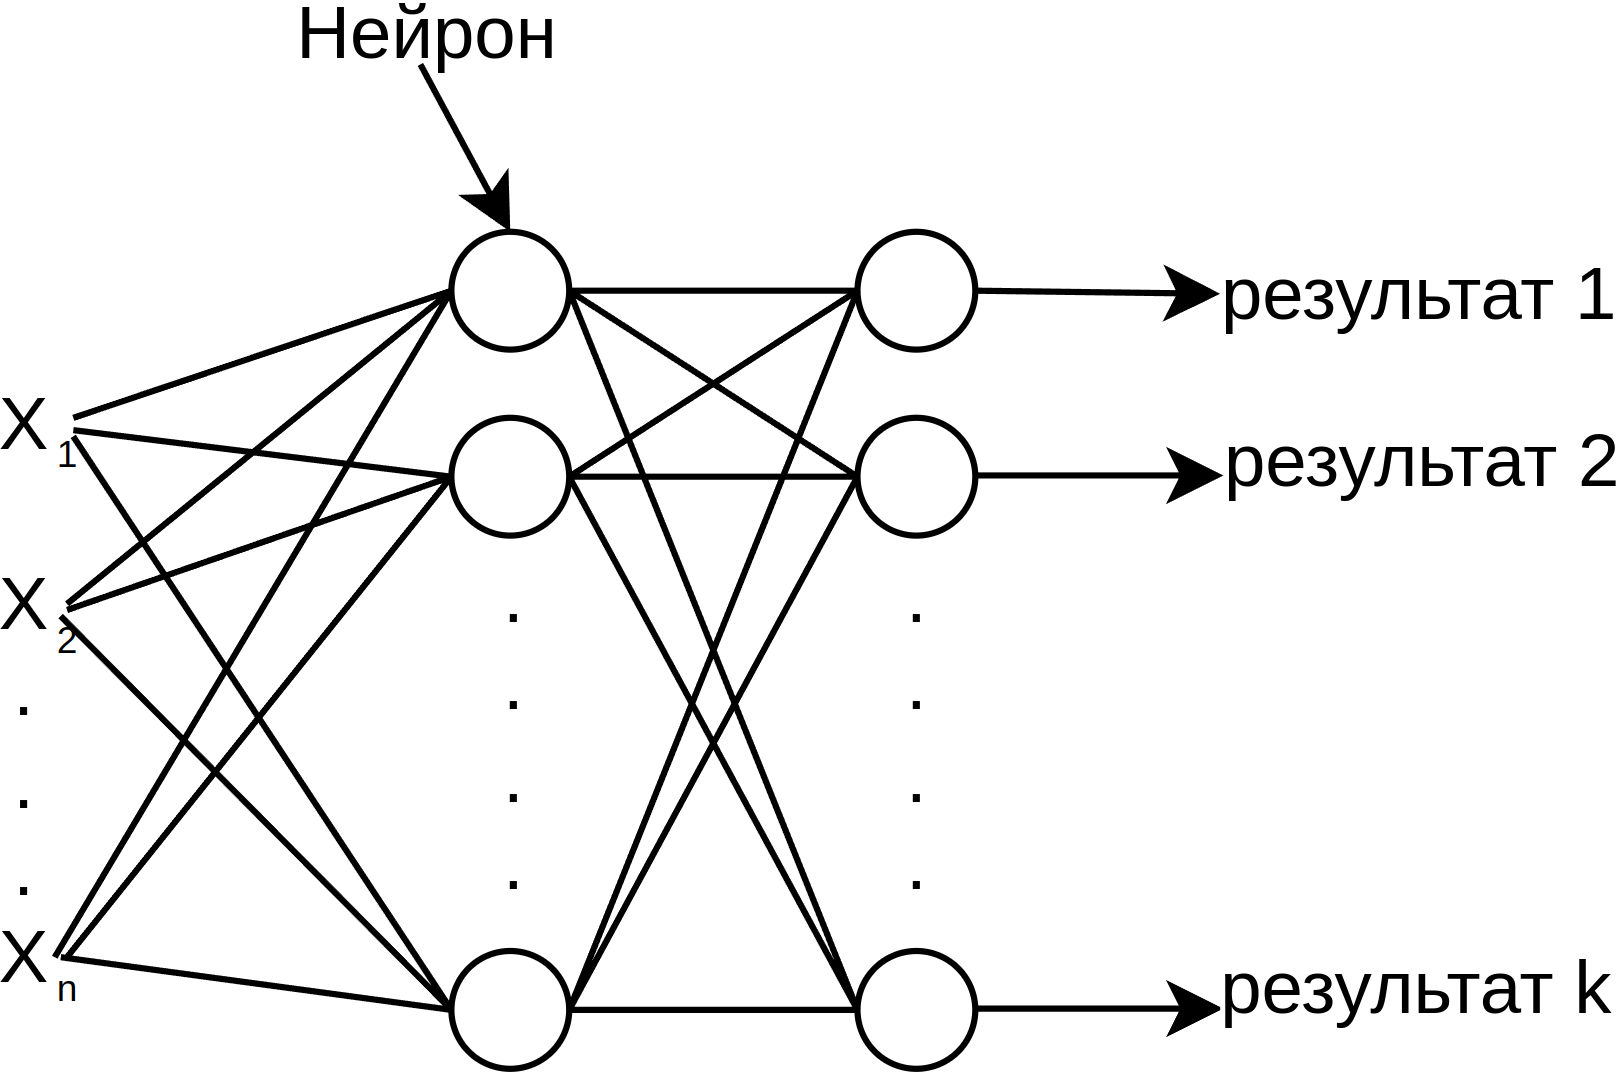
\includegraphics[scale=0.75]{Images/neural_network_architecture.png}
	\caption{Загальна архітектура повнозв'язної нейронної мережі}
	\label{fig_nn_arch}
\end{figure}

Тепер розглянемо, як працюють генетичні алгоритми. Існує багато різних варіацій генетичних алгоритмів, але основна структура наступна: першим кроком ініціалізується популяція індивідів, для задачі класифікації, кожен індивід буде класифікатором, далі розраховується фітнес функція для кожного індивіду, далі якимось чином обирається підмножина індивідів для створення наступного покоління, далі застосовуються операції мутації та кросинговеру до відібраних індивідів, далі розраховується фітнес функція для кожного нового індивіду, далі відбираються індивіди для нової популяції. Цей процес повторюється ітеративно, певну кількість ітерацій, або поки не буде виконана якась умова завершення алгоритму. Індивід може бути представлений різними способами, наприклад вектором бітів. Фітнес функція може варіюватися від задачі, наприклад, якщо індивід це вектор бітів, а задача це отримати вектор тільки з одиниць, то в якості фітнес функції може бути функція, яка розраховує кількість одиниць в векторі (в цьому випадку, чим більша фітнес функція тим більше пристосований індивід). Методів відбору для репродукції існує також багато, але ось декілька прикладів найпопулярніших: рулетковий відбір~\cite{ct2} (кожному індивіду присвоюється ймовірність з яким він може обратися для репродукції і після цього обираються індивіду, враховуючі ці ймовірності), турнірний відбір~\cite{ct3} (випадковим чином обирається групка індивідів з усієї популяції і з цієї групки для репродукції обирається той індивід у якого найкраща фітнес функція), елітизм

\section{(Назва третього підрозділу)}


Надамо деякі рекомендації щодо використання даного стильового файлу.

\begin{theorem}
Використовуйте оточення \emph{theorem} для теорем.
\end{theorem}
\begin{proof}
Для доведень використовуйте оточення \emph{proof}.
\end{proof}
\begin{theorem}
Нумерація відбувається автоматично
\end{theorem}
\begin{claim}
Використовуйте оточення \emph{claim} для тверджень.
\end{claim}
\begin{lemma}
Використовуйте оточення \emph{lemma} для лем.
\end{lemma}
\begin{corollary}
Використовуйте оточення \emph{corollary} для наслідків.
\end{corollary}
\begin{definition}
Використовуйте оточення \emph{definition} для визначень.
\end{definition}
\begin{example}
Використовуйте оточення \emph{example} для прикладів, на які є посилання.
\end{example}
\begin{remark}
Використовуйте оточення \emph{remark} для зауважень. Зверніть увагу, як 
веде себе команда \textbf{emph}
\end{remark}


\chapconclude{\ref{chap:review}}

Наприкінці кожного розділу ви повинні навести коротенькі підсумки по його 
результатах. Зокрема, для оглядового розділу в якості висновків необхідно 
зазначити, які задачі у даній тематиці вже були розв'язані, а саме 
поставлена вами задача розв'язана не була (або розв'язана погано), тому у 
наступних розділах ви її й розв'язуєте.

Якщо ваш звіт складається з одного розділу, пропускайте висновок до 
нього~-- він повністю включається в загальні висновки до роботи